%%%%%%%%%%%%%%%%%%%%%%%%%%%%%%%%%%%%%%%%%%%%

% formato FRONTE RETRO
\documentclass[epsfig,a4paper,11pt,titlepage,twoside,openany]{book}
\usepackage{epsfig}
\usepackage{plain}
\usepackage{setspace}
\usepackage[paperheight=29.7cm,paperwidth=21cm,outer=1.5cm,inner=2.5cm,top=2cm,bottom=2cm]{geometry} % per definizione layout
\usepackage{titlesec} % per formato custom dei titoli dei capitoli

\singlespacing

\usepackage[italian]{babel}

%%%%%%%%%%%%%%%%% STEFANO ADDED %%%%%%%%%%%%%%%%
% supporto lettere accentate
% queste due righe nel preambolo servono a poter utilizzare le lettere accentate in tutto il testo se no di norma si inserirebbero con \'e...
\usepackage[T1]{fontenc}
\usepackage[utf8]{inputenc}
\usepackage{hyperref} %Serve per i riferimenti
\usepackage{caption}  %Serve per le note (caption)
\usepackage{multicol}	 %Serve per usare più colonne

%%%%%%%%%%%%%%%%% ENRICO ADDED %%%%%%%%%%%%%%%%%
\usepackage{ulem} %Serve per il sottolineato
\usepackage{amsmath} %Serve per alcuni ambienti matematici
\usepackage{array} %Serve per le tabelle
\usepackage{multirow} %Seve per tabelle
\setcounter{secnumdepth}{5} %Utilissimo serve per aumentare il numero di paragrafi, si arriva fino a 5 livelli di profondità x.x.x.x.x
%GRAFICI
\usepackage{pgfplots}
\usepackage{pgfmath}
\usepackage{tikz}
%CODICE
% \usepackage{listings}
% \usepackage[cache=false]{minted} 
%\setminted{tabsize=4, breaklines, breakanywhere, linenos, mathescape,}

% \lstset{
% 	  breakatwhitespace=false,         
% 	  breaklines=true,     
% 	  basicstyle=\footnotesize\ttfamily,            
% 	  commentstyle=\color{blue}, %Indica il colore dei commenti
% 	  keywordstyle=\color{red}, %Indica il colore delle parole chiave
% 	  language=C, %Indica il linguaggio predefinito da usare
% 	  rulecolor=\color{black}, %Indica il colore dei numeri di righe
% 	  tabsize=4,
% 	  escapeinside={\%*}{*)},
% 	  morekeywords={}, %Altre parole da inserire tra le keywords. Ad esempio possiamo aggiungere do, gotttto, ecc ecc 
% }
%%%%%%%%%%%%%%%%% END OF ENRICO  %%%%%%%%%%%%%%%%

\begin{document}
%set the language of the text to italian
% !TeX spellcheck = it_IT

%%%%%%% personal commands (ALIAS):
% \newcommand{\nome_commando}[argomenti]{comando}
\newcommand{\e}[1]{$\cdot 10^{#1}$}
\newcommand{\mmax}[0]{mod\_withMax }
\newcommand{\mover}[0]{mod\_overlap }
\newcommand{\mmod}[0]{modularità modificata }
\newcommand{\nv}[0]{Node2Vec }
\newcommand{\wv}[0]{Word2Vec }
\newcommand{\cnrl}[0]{CNRL }
\newcommand{\cora}[0]{Cora }
\newcommand{\citeseer}[0]{Citeseer }
\newcommand{\LPred}[0]{Link Prediction }
%



%
%
\chapter{Implementation}
In this section, I am going to explain thanks to which method we tried to outperform the potentiality of the code of CNRL. 
\section{How the CNRL's code work}
How the code of CNRL exactly work?\\
First of all, the data are loaded from files, this includes the graph in edgelist format. After that, the graph is prepared for node2vec algorithm this is a particular method for exploring the graph, in fact, it depends on two parameters, named $p$ and $q$. The value of the two parameters allow a depth visit or something that are more similar to a breadth visit, or possibly a solution in the middle.\\
But why we walk on the graph?\\
The main idea is to start some walks (in the number of $w$), from each node of the graph (in the number of $n$). And each walk have a length not higher than the value of $l$, I said not higher because if we have a directed graph it is possible that we arrive in a sink, then the walk must be interrupted because it is not possible to walk more. Differently, if we have an undirected graph all the walks have a length of $l$ because node2vec allows a path that goes back.\\
At the end of that, we have $w \cdot n$ walks with a maximum length of $l$\\
Given the walks it is possible to obtain the community of the graph, this process is done with two different approaches, the first one is one of the most famous, named word2vec, that is going to consider the nodes' ID find in the walks like words, and then consider the walks like sentences.\\
Differently in the code of CNRL is used an algorithm created on purpose, and we have never tried to understand how it works exactly.\\
After that the partition is created, it is possible to calculate the modularity, with the algorithm that I explained in his chapter.
%
\section{Introduce of attribute}
As you can understand, CNRL's code for calculating the community use only the structure of the graph, that means, how the nodes and the edges are interconnected.\\
We note that both dataset on which we work, named Cora and Citeseer (better explained in the chapter on the experiments), have for each node a set of attribute, this can be present 1 or not 0. All those pieces of information are not considered from the CNRL's code so we decide to introduce it. The only part where we can work is before the extraction of the community given the walks and after the loading of data from the input files, this means that we can change only the generation of the walks.\\
The idea is to create in addition to the firsts walks, some other walks that manage the nodes through the attributes. When we see at the graph we can say that two nodes are near if there is a link between them.\\
When can we say that two nodes through an attribute are similar? Of course, when both share the same attribute. We can imagine that the sharing of an attribute is like an undirected link or edge, in fact, there is not any direction with the sharing. Then we can build a new undirected graph that considers the attribute and we are going to go to walk on it.
%
\section{Attribute graph}
In all the previous words we have described the graph taken from the attribute. I try now to formalize this concept.\\
First of all, we must remember that we have the original edges that we must delete, in fact, we do not want to walk on it, or the new walks will be a copy of the first ones. Then from the original graph, we preserve only the nodes, called from now N1.\\
Thanks to the reasoning done before, that if two nodes share the same attribute, they are near. We can imagine that an edge, goes or directly from a node of N1 to another. Or we can create a new set of nodes, named N2, that contain all the attributes, each attribute becomes a node.
%
\begin{figure}[htp]
	\centering
	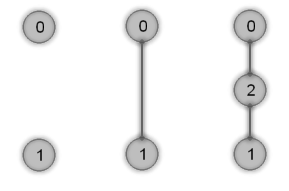
\includegraphics{images/add_att2}
	\caption{Two nodes that share an attribute, how we can link them, 1-no edge, 2-hypergraph, 3-bipartite graph}
	\label{fig:add_att2}
\end{figure}
\begin{figure}[htp]
	\centering
	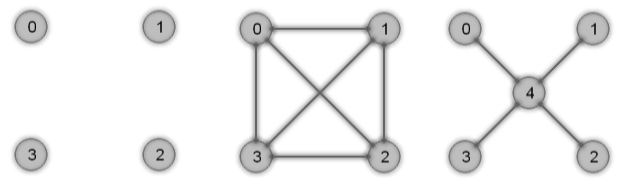
\includegraphics[width=\linewidth]{images/add_att4}
	\caption{Four nodes that share an attribute, how we can link them, 1-no edge, 2-hypergraph, 3-bipartite graph}
	\label{fig:add_att4}
\end{figure}
\\
Then exist two methods to link some nodes through the attribute. In figure~\ref{fig:add_att2} and~\ref{fig:add_att4}, there are two different examples. In both figures we have three scenes, the first one shows the nodes without any linkage, the second one shows the nodes connected directly, in the last one we have the nodes connected across another node that does the hub, this hub is the node taken from the attribute.
Is easy to understand the difference, the second scene, named hypergraph, create a complete graph, this mean that I have  $ \displaystyle\binom{n}{2}$ edges, in figure~\ref{fig:add_att4} are $ \displaystyle\binom{4}{2} = 6$, but no one node is added.\\
The third scene is a star graph that builds a bipartite graph, add a node for each attribute, but only $n$ edges, for figure~\ref{fig:add_att4} this mean that we add one node and four edges.\\
Which one we prefer?\\
It depends on the situations, if there are lots of attributes and each of these is available for a little number of nodes, probably we are going to prefer the hypergraph. If there are some attribute that is available for a high number of nodes probably we prefer the bipartite graph.\\
In fact if for example we have an attribute available for $100$ nodes this mean that with the bipartite graph we add $1$ node and $100$ edges, for the hypergraph we add zero nodes but $ \displaystyle\binom{100}{2} = 4950$ edges.\\
For this reason, we have chosen for use the bipartite graph.\\
To note that when we walk on this new graph we save in the array of walks for both type of nodes, then after walking we must delete the ID of the nodes belonging to the attributes. Because the future steps of the algorithm must not know the existence of the bipartite graph.
%
\subsection{Name of bipartite graph}
I would like to explain where this name does come from. The graph is called bipartite because there are two set of nodes, the nodes that before I called N1 (original nodes) and N2 (nodes from attribute). Every edge of the graph goes from a node of N1 to a node of N2 and vice versa. There is no one edge that goes from N1 to N1 or from N2 to N2. This is perfect for our situation if we had two nodes of N1 linked this would mean that we have not deleted the original edges if we would have two nodes of N2 linked this would mean that we have done an error, two attributes can not be linked.
%
\subsection{Name of hypergraph}
I would like to explain where this name does come from. The hypergraph do not have simple edges but have hyperedges, the normal edges have two endpoints and both are nodes, so its possible to represent it with a line. Differently, the hyperedges do not have two endpoints but potentially an infinite number of endpoints, this allows that a hyperedge link more than two nodes directly. If you want to represent an hyperedges on a normal undirected graph this mean that, if the hyperedges link directly 5 nodes we must replace it with a complete graph on this 5 nodes so we use $ \displaystyle\binom{5}{2} = 10$ normal edges.

Note that, this is exactly our situation, in fact, an attribute link the nodes to which it belongs directly, so we can imagine that for each attribute we are going to create a hyperedge on his nodes.
%
%

\section{Build graph - example}
In this section, I am going to show how a graph is transformed from the simple structure and the attributes to a hypergraph or to a bipartite graph.\\
%
\begin{multicols}{2}
	\begin{center}
		\begin{tabular}{|l|cc|}
		\hline
		ID&\multicolumn{2}{c|}{attributes ID}\\
		\hline
		1&11&\\
		2&11&12\\
		3&10&12\\
		4&11&13\\
		5&11&12\\
		6&12&13\\
		7&13&14\\
		\hline
		\end{tabular}
		\captionof{table}{For each node, there are the attributes ID that it has}
		\label{tab:7_ID_to_att}
		%
		\begin{tabular}{|l|cccc|}
		\hline
		att&\multicolumn{4}{c|}{node ID}\\
		\hline
		10&3&&&\\
		11&1&2&4&5\\
		12&2&3&5&6\\
		13&4&6&7&\\
		14&7&&&\\
		\hline
		\end{tabular}
		\label{tab:7_att_to_ID}
		\captionof{table}{For each attribute, there are the nodes ID that it has}
	\end{center}
\end{multicols}
%
%
\begin{figure}[htp]
	\centering
	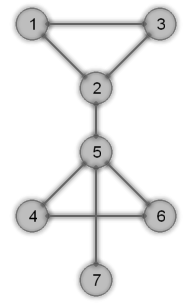
\includegraphics{images/7transform_str}
	\caption{The structure representation of the graph}
	\label{fig:7transform_str}
\end{figure}
%
%
In figure~\ref{fig:7transform_str} we can see the structure of the graph. In table~\ref{tab:7_ID_to_att} we can see that for each node is represented the ID of the attributes that it has. At the opposite in table~\ref{tab:7_att_to_ID} for each attribute, are represented the ID of the nodes that have it.\\
Then now it is possible to create the two graphs.
%
\begin{figure}[htp]
	\centering
	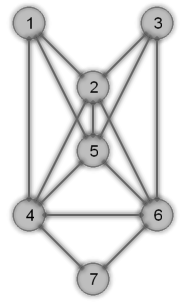
\includegraphics{images/7transform_hyper}
	\caption{The representation of the hypergraph}
	\label{fig:7transform_hyper}
\end{figure}
\\
First, we look at the hypergraph shown in figure~\ref{fig:7transform_hyper}.
\begin{itemize}
	\item  we can see that some edges are no more present, two examples are $(1,3)$ and $(5,7)$, some other before was deleted and after they are replaced
	\item  the nodes that share the same attribute build a complete graph, two example are $[1,2,4,5]$ with the attribute $11$ and $[4,6,7]$ with the attribute $13$
	\item  if only one node has a particular attribute this does not create an edge, this is the case of the two attributes $10$ and $14$
\end{itemize}
%
\begin{figure}[htp]
	\centering
	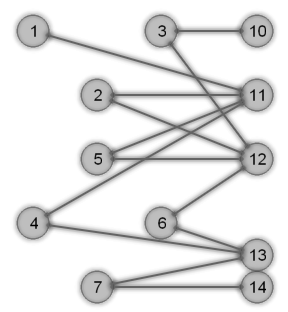
\includegraphics{images/7transform_bipartite}
	\caption{The representation of the bipartite graph}
	\label{fig:7transform_bipartite}
\end{figure}
%
We look now a more complex situation, the bipartite graph shown in figure~\ref{fig:7transform_bipartite}. It is not easy to see what happen.\\
The nodes from 1 to 7, on the left, are the original ones the nodes from 10 to 14 (higher equal than 10), on the right, are the new ones created from the attributes. 
\begin{itemize}
	\item the nodes on the left and the nodes on the right are separate are the two sets of which I spoke before N1 and N2
	\item all edges cross the middle of the graph, go from left to right
	\item all the edges present in the original graph are no more present, we have deleted all of them
	\item the nodes that share the same attribute build a star graph, two example are $[1,2,4,5]$ with the attribute $11$ and $[4,6,7]$ with the attribute $13$
	\item  if only one node has a particular attribute this do not do difference, in fact, the two attributes $10$ and $14$ are anyway linked to the left part
\end{itemize}
%
%
%
%\end{document}
